\documentclass{article}
\usepackage[round]{natbib}
\usepackage{amsmath,amssymb,amsfonts}%
\usepackage{geometry}%
\usepackage{color}
\usepackage{graphicx}
\usepackage{authblk}
\usepackage{nameref}
\usepackage[right]{lineno}

\begin{document}

\linenumbers
\title{What is an Ancestral Recombination Graph?}
% First authors
\author{Author McAuthorface}
% Corresponding

\maketitle

% JK: this is a rough first pass for a slightly different paper. Needs
% substantial revision.
\begin{abstract}
It has recently become possible to infer genetic ancestry in the presence of
recombination at scale for the first time. This has created exciting
possibilities, with many downstream applications based on
these inferred genealogies. The inferred genetic ancestries are usually
referred to as Ancestral Recombination Graphs, or ARGs. Although initially well
defined as a graphical representation of the coalescent with recombination
stochastic process, the interpretation has become unclear as it is now
also understood to represent a particular realisation of a genetic
ancestry.
Inference methods do not all infer the same information:
although all output marginal trees along the genome, there is a great deal of
variation in how much information of the relationships between the trees is inferred
and retained. An important programme of work over the coming years is to
develop and refine ancestry inference methods, assessing the relative strengths
and weaknesses of the various approaches. Using the blanket term ARG hides the
important differences in the approaches, and hampers our ability to compare and
improve inference methods. In this paper we discuss the different approaches we
may use to encode genetic ancestry, and of the differing amounts of information
about the ancestral process that we can represent and hope to observe. We
classify existing inference methods according to the type of ancestry they
infer, and discuss the strengths and weaknesses of the inferred structure for
downstream applications.
\end{abstract}

\textbf{Keywords:} Ancestral Recombination Graphs

\section*{Introduction}

% HYW: this is a rough first pass, aiming to be concise. We should flash out the "recombination" aspect of ARGs here a bit, I think

For a long time, the Ancestral Recombination Graph (ARG) has been an object of
fascination to those interested in theoretical evolutionary genetics, as it
captures all knowable genetic history of a collection of individual genomes.
Recently advances in our ability to infer ARGs has led to a resurgence of
interest in this field. However, these have also given rise to certain
terminological confusion, which we aim to clear up in this paper.

One major source of confusion is the use of the term ``ARG" to refer to both a
backwards-in-time generative process (Griffiths) and a structure which can be
created by that process
\citep[e.g.][]{minichiello2006mapping,mathieson2020ancestry}.

\section*{Ancestral graphs and stochastic processes}

% See https://github.com/tskit-dev/what-is-an-arg-paper/discussions/13
% for discussions on this section

The simplest prominent example of genetic ancestry generated by a stochastic process
is the coalescent process \citep{kingman1982coalescent,kingman1982genealogy,
hudson1983testing, tajima1983evolutionary}, which describes the random
ancestral tree at one non-recombining locus obtained by sampling a relatively
small number of individuals at random from a large population.

In a recombining organism, the genetic ancestry of a longer segment of DNA is 
no longer described by a single tree. Instead, ancestral relationships in a
sample can be represented by a sequence of correlated, marginal trees along the
genome. The Ancestral Recombination Graph (ARG) was introduced by
Griffiths~\citep{griffiths1991two,griffiths1997ancestral} as a branching-coalescing 
stochastic process whose realisations are graphs which into which all of the
marginal ancestral trees are embedded. Coalescences encode common ancestry
as they do in the coalescent, while branching events encode points at which a
marginal tree changes from one position along the genome to the next.
%note-jk: could nitpick this in that diamonds don't generate tree "changes" as such. Maybe tweak this on the next round of revision?

% jk-note: this isn't quite right I think, as it's muddling the distinction between a graph stochastic process 
% definition with the graph as the encoding of the marginal trees. 
There are several formulations of the ARG, which vary by
the amount of extra information they capture beyond a minimal representation
of all marginal trees. Two prominent examples are the ``big''
ARG~\citep{ethier1990two}, which has a particularly simple specification as a
stochastic process but is computationally infeasible, and the ``little ARG''
traversed by Hudson's algorithm~\citep{hudson1983properties}, which
has a more complex state space and dynamics but can be implemented with 
a more manageable runtime and memory footprint. An efficient simulation
implementation has become available only recently \citep{kelleher2016efficient},
prior to which state-of-the-art simulators were based on the so-called sequentially
Markovian coalescent (SMC) \citep{mcvean2005approximating}, which delivers
performance gains by disallowing mergers which would result in trapped
non-ancestral material. An alternative restricted model is
\texttt{ClonalFrame}  \citep{didelot2007inference}, which fixes one distinguished
tree and disallows recombination in any other marginal tree.

Similar graph encodings have also been introduced to model other mechanisms
which change the local ancestral tree along the genome, such as gene
conversion~\citep{wiuf2000coalescent} and
horizontal gene transfer~\citep{baumdicker2014infinitely}.

The idea of using branching-coalescing stochastic processes 
to model genetic ancestral trees has also found application in natural selection.
The Ancestral Selection Graph (ASG)~\citep{krone1997ancestral,neuhauser1997genealogy}
uses dynamics identical to the ``big" ARG to simulate an ensemble of correlated
potential ancestral trees. Weak genic selection is incorporated by sampling a 
true ancestry from the ensemble in a non-uniform way.
There is no ASG analogue of the more computationally tractable ``little" ARG,
though some gains in tractability can be made by considering typed 
lineages~\citep{etheridge2009coalescent} or by leveraging perfect simulation
techniques when recurrent mutation is present\citep{fearnhead2001perfect}.
Extensions of the ASG have been developed to frequency-dependent 
selection~\citep{neuhauser1999ancestral, gonzalezcasanova2018duality},
unlinked chromosomes~\citep{fearnhead2003ancestral}, recombining
loci whereupon branching is due to both selection and
recombination~\citep{donnelly1999genealogical}, and high fecundity 
reproduction~\citep{gonzalezcasanova2018duality, koskela2019robust}.

In the theoretical literature, ancestral graphs such as the ARG refer to the
ancestral \emph{process} rather than the outcome of a process.

\section*{The ARG as a structure}

\citep[e.g.][]{minichiello2006mapping,mathieson2020ancestry}.

\begin{figure}
\vspace{5em}
\caption{\label{fig-pedigree-and-arg}
The (unannotated) ARG is closely related to the pedigree
graph, where each ``individual'' node is replace by two ``genome''
nodes, and edges between parents and children are only included if there is
transfer of ancestral material. We usually only include nodes in an ARG
that affect our sample, so that, for example, individuals that are ancestral
to only one sampled genome are not included.}
\end{figure}


% HYW: this is a rough first pass. We should take care not to assume that the tree sequence
% approach is the only encoding

The other use of the the term ARG, and the one for which we suggest the term be
reserved, is to describe the *structure* resulting from the genetic process of
inheritance. This structure, like any other graph, consists of *nodes*
connected by *edges*. In the context of genetics, the nodes represent (haploid)
genomes, and the edges represent paths of inheritance. Although for theoretical
purposes a graph like this can be created by backwards-in-time simulations
using the CwR, in reality it is created forwards-in-time, as a population
evolves.

Since genetic inheritance is unidirectional, the edges in this graph structure
are *directed*, with a "parent" and "child" node. Moreover, there is a strict
temporal order, so that children cannot be their own parents: in other words,
there are no cycles in the graph, and it is technically a form of "directed
acyclic graph" (DAG).

% HYW: NB: worded carefully below, as it should also be possible to encode ARGs even if there is not a single fixed coordinate system

There is one key feature which distinguishes an ARG for other graphs. Although
a genome (graph node) may have more than one parent, the particulate nature of
genetic inheritance means that each letter in the genome can only come from a
*single* parent. Hence if we compare the equivalent letters from multiple
extant genomes, their paths of inheritance must form a *tree* (which,
incidentally, is why phylogenetics plays such an important role in evolutionary
theory). As we shall argue, the ability to generate these "local trees" from an
ARG is of key importance.

When describing an ARG, the primary issue, from a practical point of view, is
how to annotate the graph with the details of which piece of genome has come
from which parent. There are two possibilities: the annotations can be
associated either with the nodes, or with the edges.

\begin{figure}
\vspace{5em}
% NB: not clear if this figure is better off on its own or should be
% merged with the pedigree one.
\caption{\label{fig-arg-annotations}
The specific path through the ARG for a given genome position (and therefore
the local genealogical tree) cannot be determined without annotations
to the graph. (A) The classical Griffiths approach annotates recombination
nodes with the corresponding breakpoint. (B) We can equivalently
annotate the \emph{edges} with the genomic intervals carrying ancestral
material. Edge annotations are somewhat more general, and have
significant computational advantages.}
\end{figure}

\subsection*{Node annotated recombination}

In the original (Griffiths) formulation, nodes which have multiple parents are
annotated with a breakpoint, representing a genomic position. The genome
lying to the left of that position is then taken to come from one parent, while
the genome lying to the right is taken to come from the other parent. This is
an elegantly concise encoding of the parental source, and is used, for example
in the ARGweaver .arg format. However, it suffers from three principal
drawbacks:


1. It assumes only a single breakpoint per node: problematic for representing
e.g. gene conversion or multiple chromosomes (but this could be circumvented by
having multiple breakpoints)
2. Nodes can only have a maximum of 2 parents. At
first sight, this seems a reasonable limitation, but it turns out that it can
be helpful to collapse multiple nodes into one, which potentially results in
more than two parents for any given node (see section XXXX)
3. Generating local
trees from such an encoding is time consuming (XXX describe *how* time
consuming - i,e. scaling properties with number of nodes - and why this is,
theoretically)

\subsection*{Edge annotated recombination}

An alternative approach to annotating nodes with the parent of origin of each
section of genome is to annotate each edge with the genomic region which is
inherited via that route. This approach was first introduced by Kelleher et al
(cite msprime paper) and now forms the basis of a comprehensive software
library.

% HYW: should discuss the link to biology & mitosis/meiosis: a "node" is
% strictly a cell - it is shorthand to associate it with an "individual"

\begin{figure}
\centering
\vspace{5em}
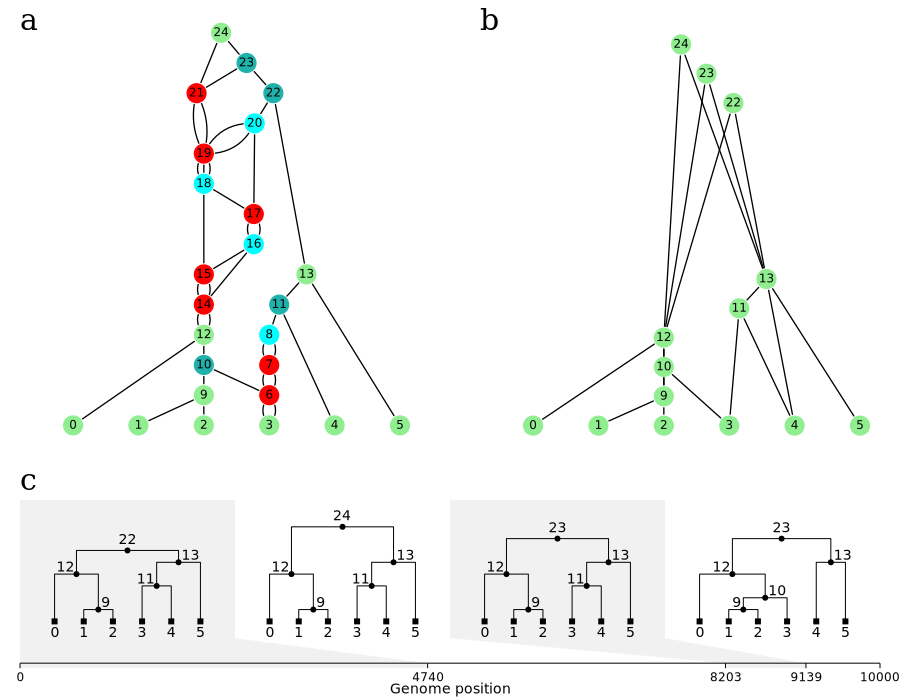
\includegraphics[width=\linewidth]{illustrations/ARG_recomb_node_deletion}
\caption{\label{fig-recombinati on-nodes}
Recombination nodes are optional in an edge-annotated ARG. (a) A simulated
ARG including all recombination nodes (red). (b) The same ARG having removed both
recombination nodes and nodes of common ancestors in which no genetic
lineages coalesce (cyan). (c) The sequence of trees corresponding to (b): if we were
to plot out the trees corresponding to (a) we would have more trees, but the topologies
and MRCA nodes at each genomic location would be identical. For clarity, nodes are
plotted by ranked time rather than true time on the y-axis.
% HYW: note that we also truncate nodes for portions in which they are unary,
% so that nodes which are coalescent nodes over only some of their length
% (blue-green) become coalescent nodes over their entire length (green). This
% can, however, throw away some useful information, for example node 4 has
% only a single parent edge in (a), but 2 parent edges (one of which appears
% to bypass node 11) in (b). In fact, this edge should go through node 11, but
% there may be no way to detect this from real data.
}
\end{figure}


\section*{ARG inference methods}
Using the terminology developed here to classify ARGs, we review methods developed
to infer ARGs. We focus our attention on some recent methods and discuss the
properties of the ARGs inferred.

The ARG has been used as a model for recombining DNA sequence data essentially
since it was first formulated. Early methods focused on finding parsimonious
ARGs consistent with a given set of
sequences \citep{hein1990reconstructing, lyngso2005minimum}.
However, identifying the most parsimonious ARG for a given sequence data set
is NP-hard \citep{wang2001perfect}, and subsequent methods have resorted to
various heuristics \citep{fallon2013acg, hein1993heuristic, ignatieva2021kwarg, 
kelleher2019inferring, minichiello2006mapping, mirzaei2017rent,
parida2008estimating, song2005efficient, thao2019hybrid, zhang2021biobank}. 
The scalability of these methods varies substantially based on the heuristic in use
and the underlying data structure, but the most efficient methods can be practically
used on megabase scale data and tens of thousands of samples under human-like
parameters \citep{kelleher2019inferring, zhang2021biobank}.

An alternative approach is to treat the ancestry as a latent parameter to be averaged out
by Monte Carlo methods, based either on importance sampling 
\citep{griffiths1996ancestral, fearnhead2001estimating, jenkins2011inference} 
or MCMC \citep{kuhner2000maximum, nielsen2000estimation, wang2008bayesian}.
These methods invariably operated on a representation of the ``little ARG", typically
generated until the grand MRCA. They are extremely computationally expensive,
and applicable to at most hundreds of samples consisting of tens of kilobases with
human-like parameters.

Due to the computational expense of sampling ``little ARGs", state-of-the-art
Monte Carlo methods typically rely on cheaper, approximate models.
The most prominent examples are \texttt{ARGWeaver} \citep{rasmussen2014genome}
and \texttt{Arbores} \citep{heine2018bridging}. The former also utilises a time
discretisation approximation, but scales to dozens of mammal-like genomes.
The \texttt{ClonalOrigin} method \citep{didelot2010inference,
medinaaguayo2020speeding} uses the \texttt{ClonalFrame}
model and data structure, though it is not as scalable as \texttt{ARGWeaver}.

A very recent MCMC method called \texttt{ARGInfer} has resulted in the first
improvement in the scalability of Monte Carlo methods for the exact ARG model 
by making use of the tree sequence representation of marginal trees, suitably enriched
to facilitate the computations needed for MCMC sampling \citep{mahmoudi2021inference}.
While not competitive with the scalability of \texttt{ARGWeaver}, \texttt{ARGInfer} extends
the feasible range of sequence lengths by at least an order of magnitude when
compared with methods which sample realisations of the exact ``little ARG".


\begin{figure}
\vspace{5em}
\caption{\label{fig-inferred-args}
ARGs inferred by different methods from a small dataset. Notes about these
ARGs.
}
\end{figure}

\bibliographystyle{plainnat}
\bibliography{paper}

\end{document}
